% SPW comments: put in right place
%First of all, I think the additional spectra of "nucleus" and "north" needed to be introduced back in Sec 2.  Presumably "bulge" is the usual 20"x30" region.  You give north and nucleus in pixels, but what are they in arcsec?  Pixels differ between SL and LL.  I'd like to see the two small regions included as table rows and in Fig 8/9 with PAHFIT, just like all the other spectra.  The main part of Fig 15 can remain as is, though probably the ordinate should be logarithmic.
%
%As to tables, I'd consolidate 1, 2, and 5 into a single table.  Add rows as appropriate for "nucleus" and "north", and give their dimensions in a footnote.  I'm not sure whether to present Fig 14 in Sec 2, but that's probably a good idea.  In Fig 14, make ticks on the vertical axis an integer number of arcsec (probably 2 or 4).
%
%When the comparison samples are introduced in Sec 4, say a few words about what they are and how they were selected.
%
%Sec 4.1 par 1: omit
%
%Sec 4.1 par 3: atomic lines need ionizing photons.  The regions observed were not selected to have H II regions in them, and they will have random amount of H II and therefore of atomic lines.  I don't think more needs to be said, but perhaps someone else will have some clever analysis.
%
%Sec 4.2 par 1: need a few references for those "many studies."  Use a review or summary article if there's a good one.
%
%Sec 4.2 par 2/3: explanation of metallicity methods is confusing.  If no one else volunteers, I can look back at the references and try to figure out a clearer explanation.  Let me know if you want me to do that.
%
%Sec 4.3 par 3: are the nucleus and north sources spatially resolved, or are they consistent with point sources?
%
%Sec 4.2 par 4: while there's no metallicity dependence, 3 of 8 regions have very low PAH.  Which regions?  Any idea why?  Is it just stellar light contamination, or is something fundamental happening?
%
%Sec 4.3 par 5: luminosity needs a sentence or maybe two at most, not a par.
%
%Fig 11/12: combine into one figure with three panels.  Caption should define what features are being plotted, explain triangles, and (briefly) explain the comparison samples.  Some points in Fig 11 are hard to see; maybe use open symbols or something for the comparison regions.  Reduce clutter by labeling fewer ticks.
%
%Sec 5: all we really need to say about ISO is that the newer reduction with zodiacal emission removed makes ISO agree with IRS.  (Was that really the only change, or was there something else different?  I'm surprised the Zodi would hide narrow features.)
%
%Appendix can go in Sec 3, perhaps as a footnote.
%

\subsection{PAH intensities}
\label{sect:pah_ratios}

Both the 6.2 and 7.7~$\mu$m features are thought to be coming from ionized PAHs and the 11.3~$\mu$m feature is from neutral PAHs. Therefore we expect to see a correlation between the intensities of 6.2 and 7.7~$\mu$m PAH features normalized by the 11.3~$\mu$m feature. In Figure \ref{PAHlines} we compare the PAH flux ratios of 7.7/11.3  and 6.2/11.3 features. The figure shows a good correlation between these two PAH line ratios and is consistent with that of SINGS sample shown by \citet{Smith:2007lr}. This correlation has also been reported in \citet{Galliano2008} and \citet{Vermeij2002}. This provides evidence that the PAH emission from M31 is not unusual. 

\begin{figure}
\centering
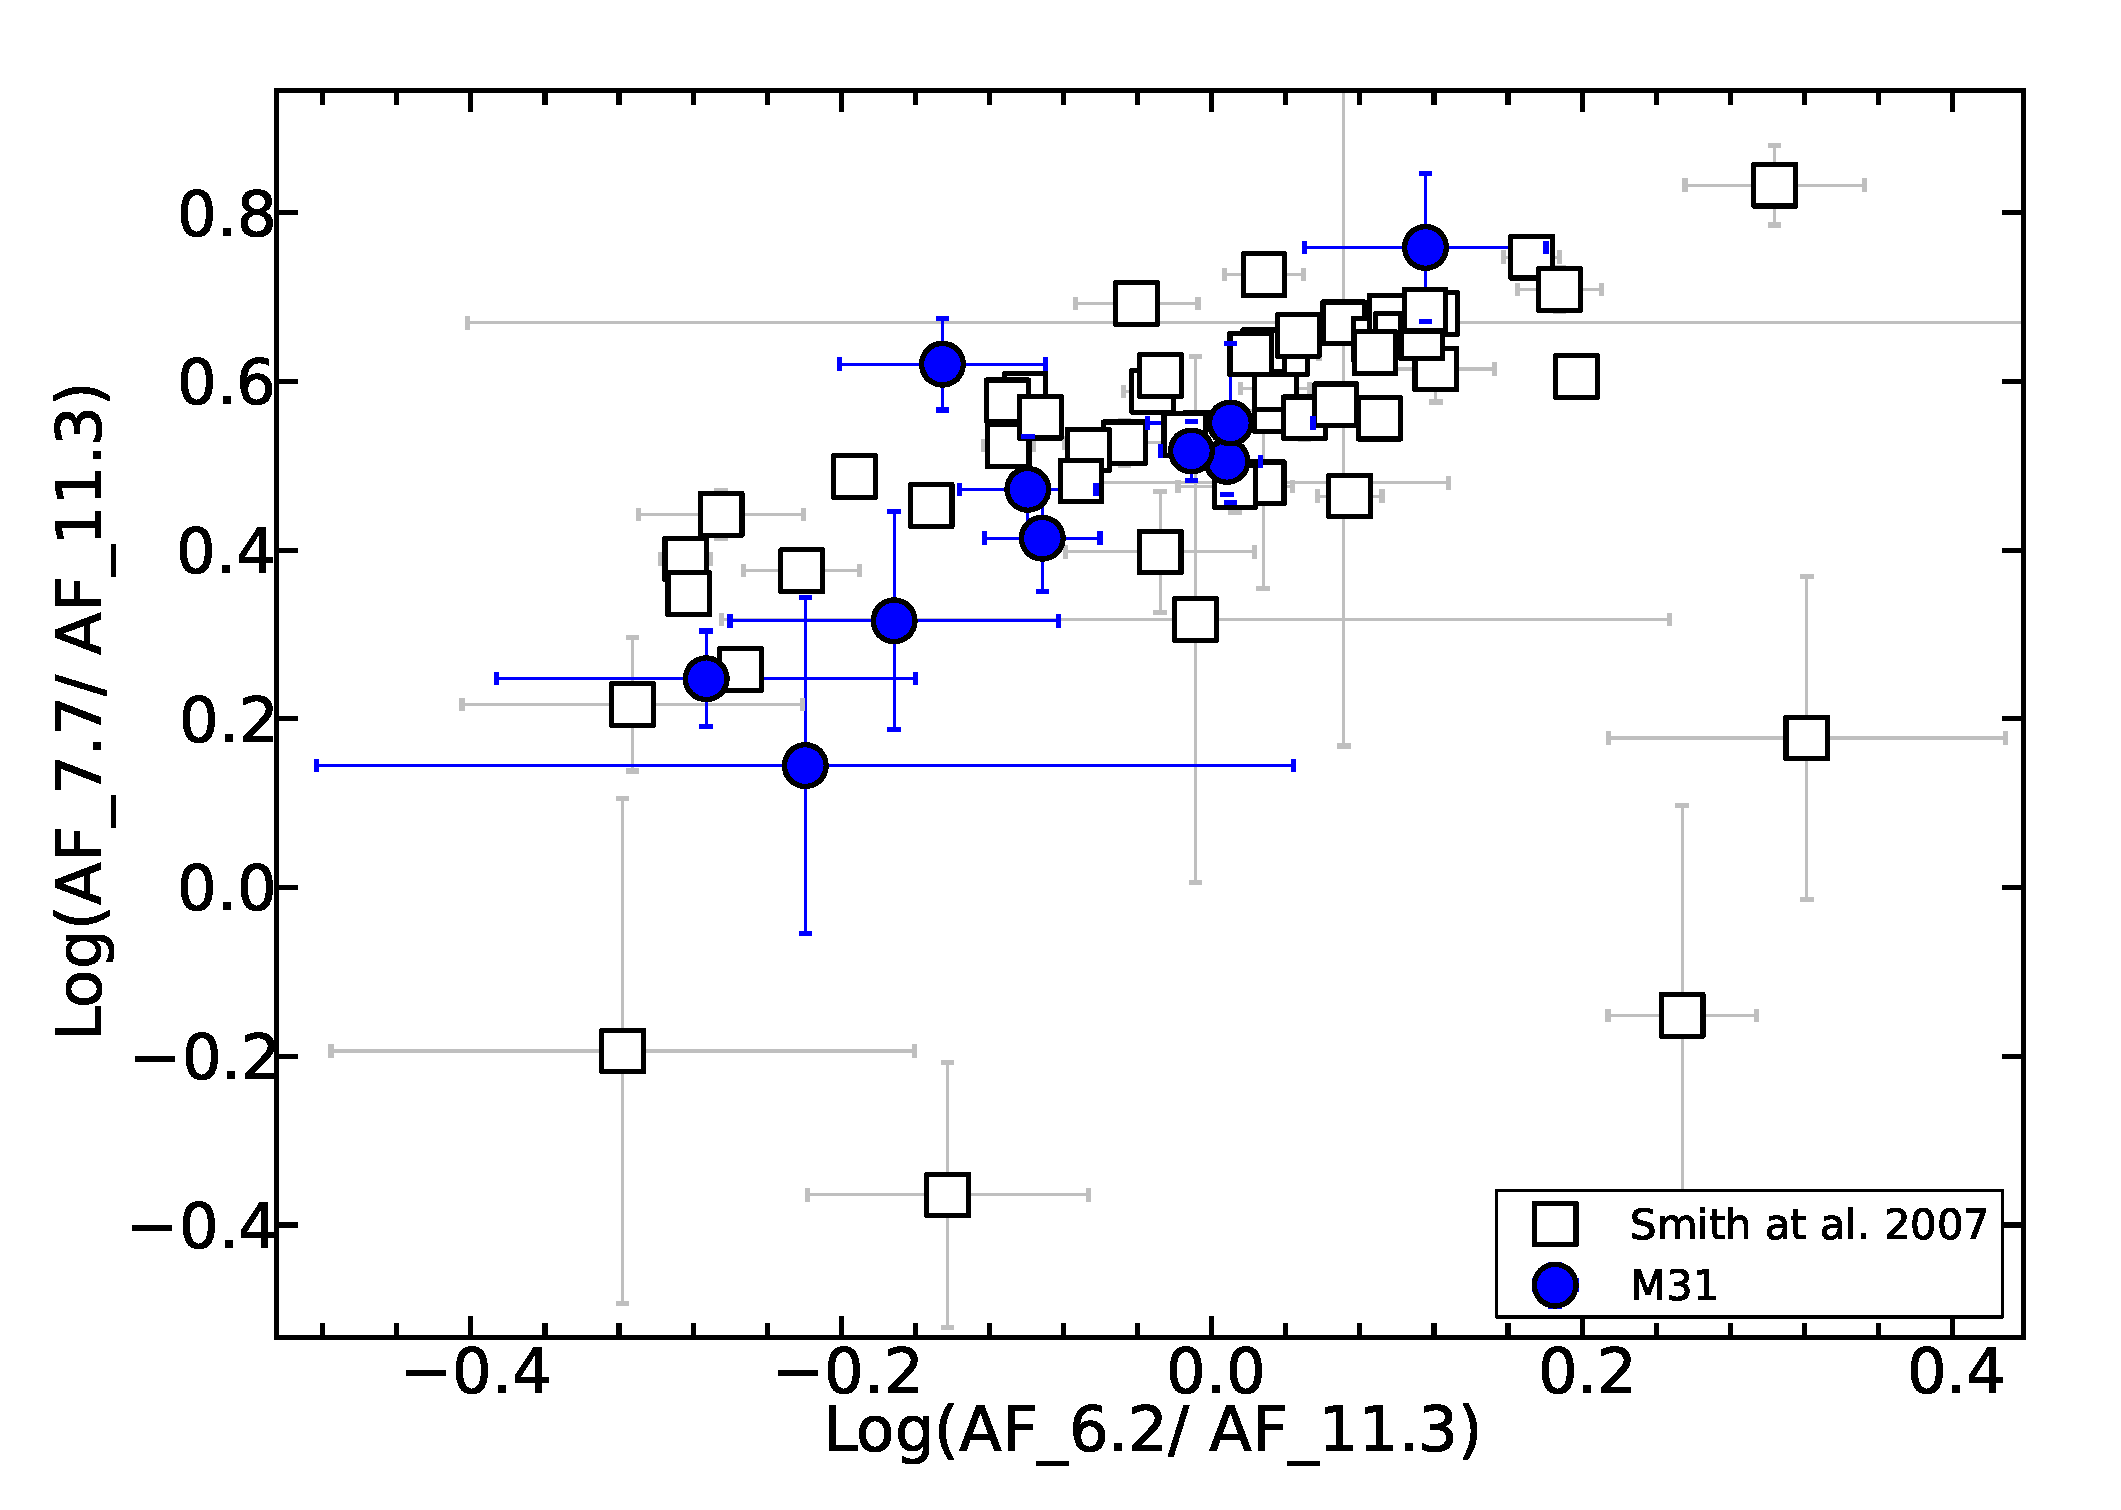
\includegraphics[scale = 0.25]{./SINGSnMy.eps}
\caption{Flux ratios for PAH features (7.7/11.3 versus 6.2/11.3) for 10 regions in M31.}
\label{PAHlines}
\end{figure}

\subsection{Aromatic equivalent widths versus radiation hardness}
\label{sect:eqw_rh}

\begin{figure}
\centering
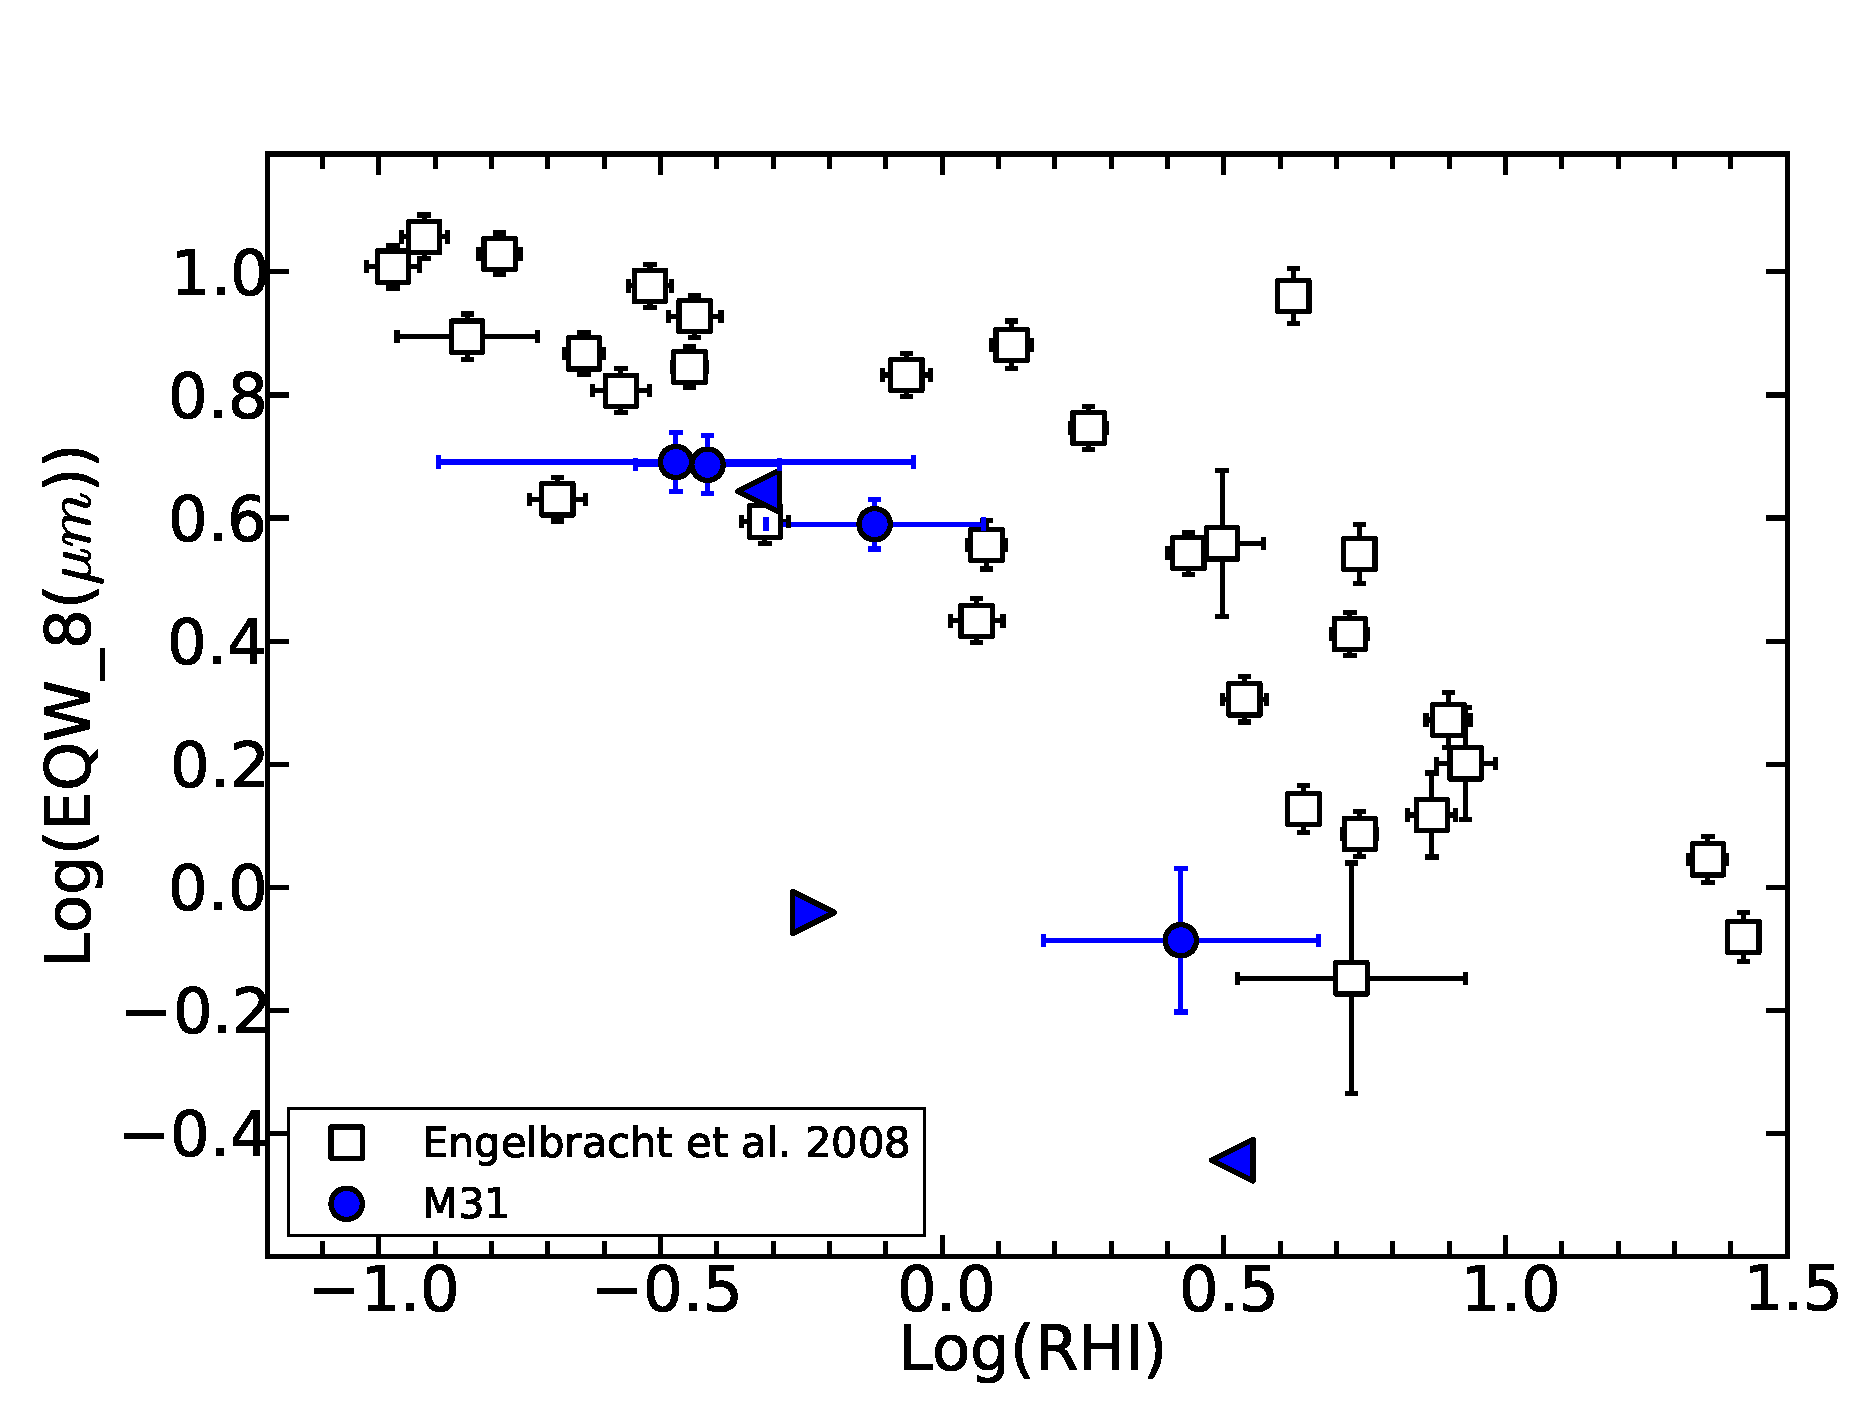
\includegraphics[scale=0.25]{./englvsmy.eps}
\caption{Equivalent widths of the 8~$\mu$m aromatic feature versus radiation hardness index (RHI) for the M31 sample (blue). 
Open squares represent the starburst sample from \citet{Engelbracht_2008}. 
Here the 8$\mu$m feature is a combination of the 7.7, 8.3 and 8.6~$\mu$m PAHFIT components. 
Triangles represents the upper and lower limits.}\label{II}
\label{englII}
\end{figure}

\begin{figure}
\centering
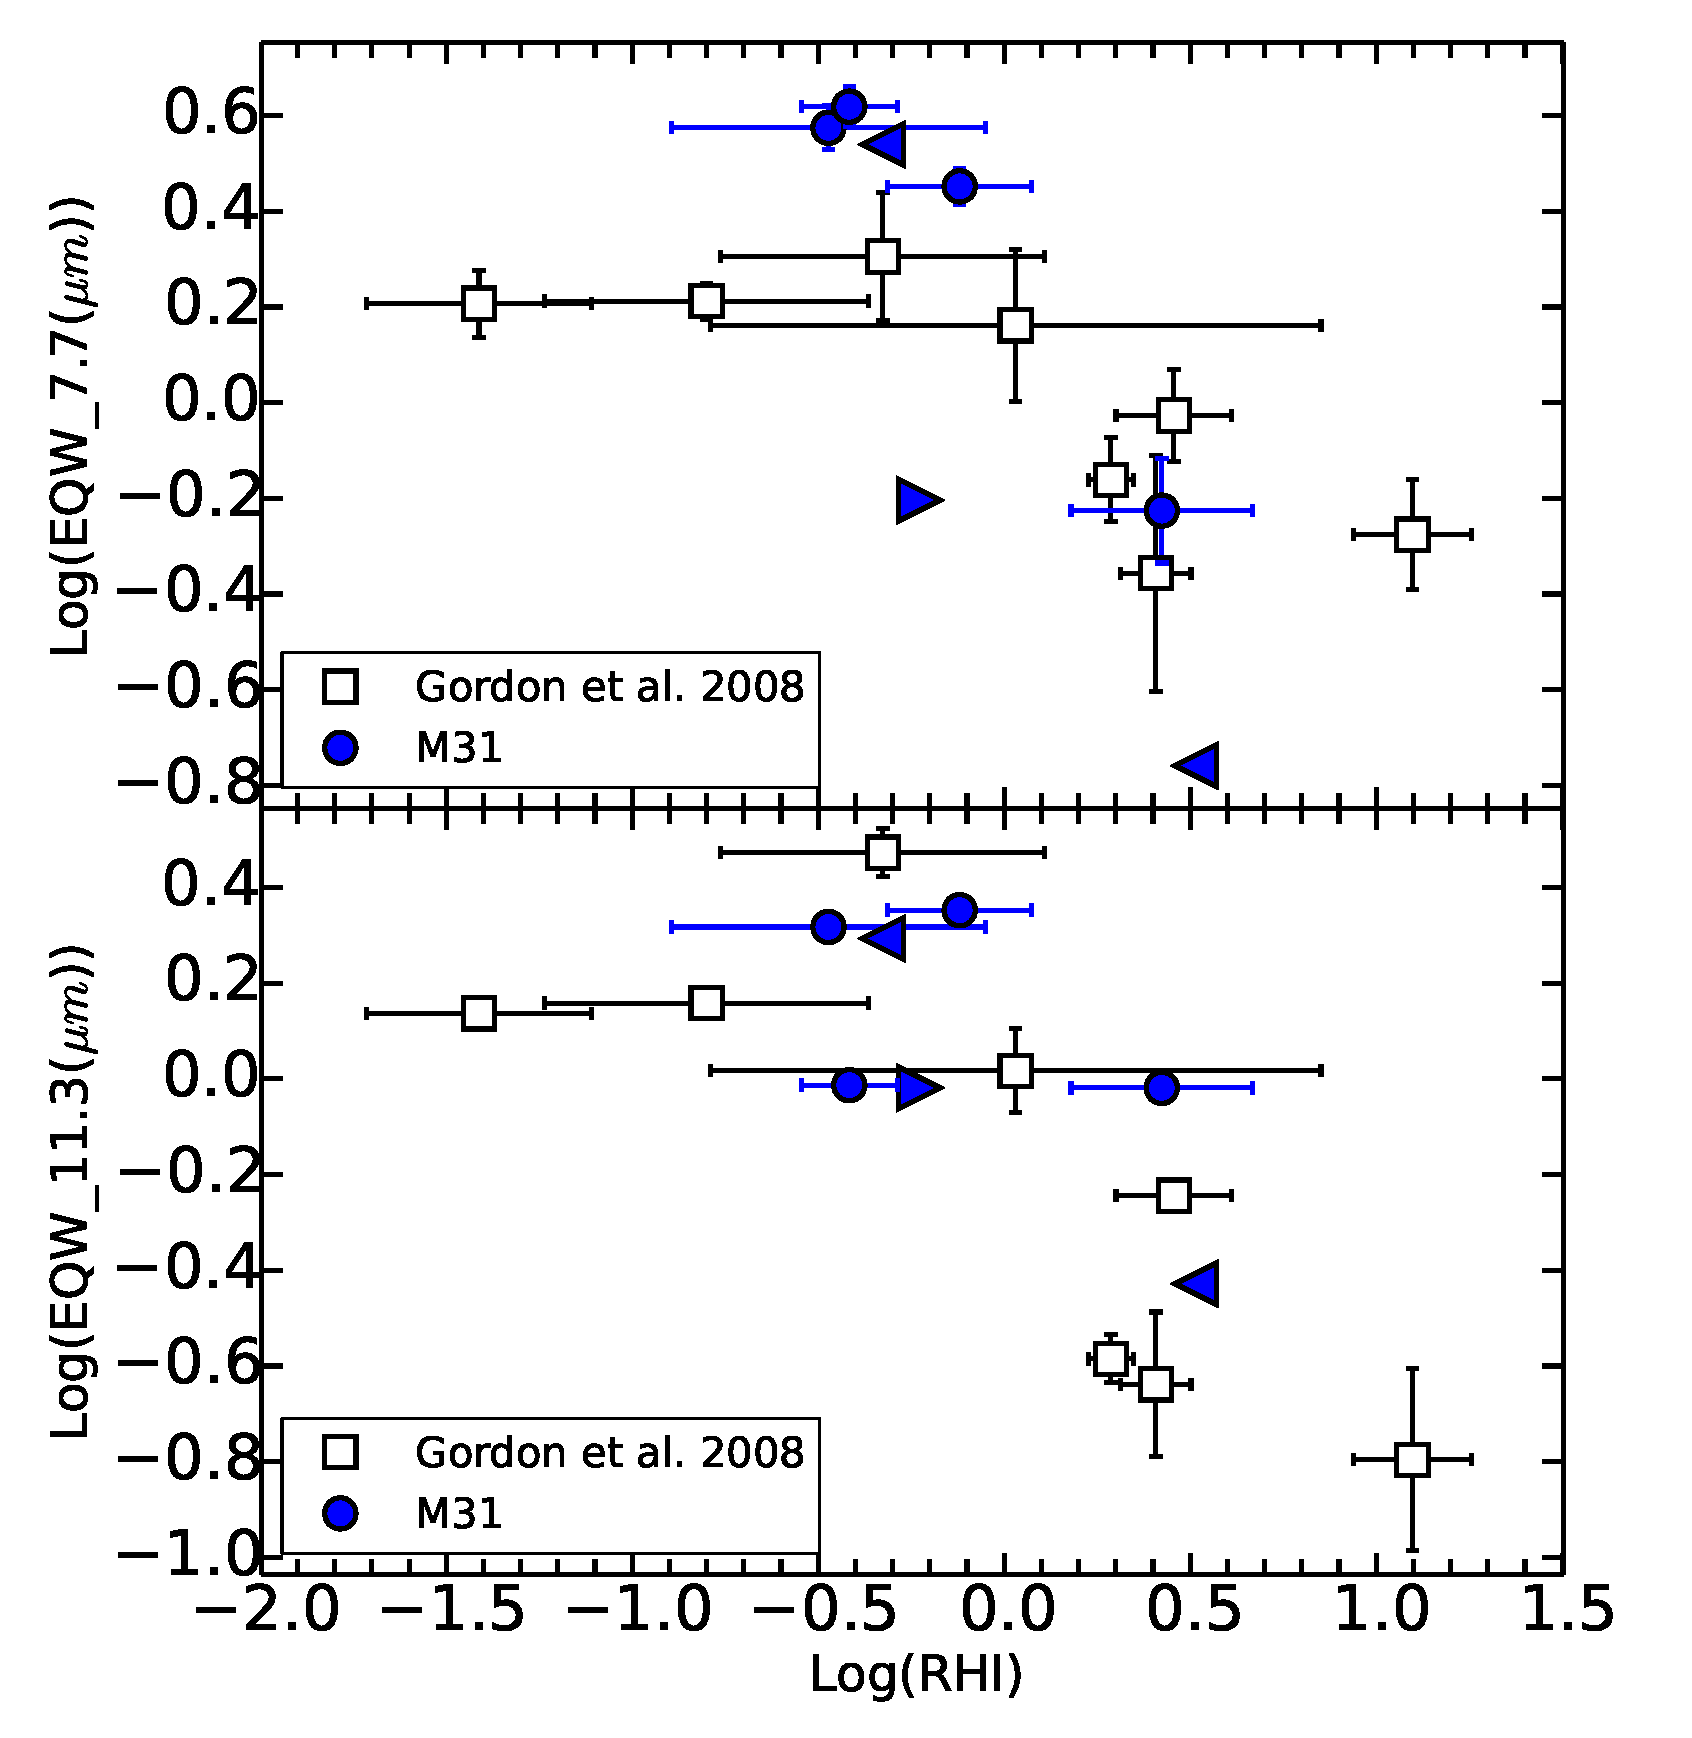
\includegraphics[scale=0.30]{./Gordvsmy.eps}
\caption{Equivalent widths of the normalized 7.7~$\mu$m aromatic feature (top panel) and 11.3~$\mu$m aromatic feature (bottom panel) versus 
radiation hardness index (RHI) for the M31 sample. Open squares represent the data from M101 by \citet{Gordon:2008lr}. 
The normalization was done by dividing each EQW by the weighted average over all regions in the respective samples. Triangles are the upper and lower limits.}
\label{gordII}
\end{figure}

As mentioned in the introduction, aromatic equivalent widths tend to show an inverse correlation with radiation hardness. We used the radiation hardness index (RHI) values calculated using the method described in Section~\ref{sect:atomic} to study how the EQW values from our sample agree with this.
The equivalent widths of the PAH features are compared with RHI in Figures \ref{englII} and \ref{gordII}.
For reference, we have added this to the starburst sample of \citet{Engelbracht_2008} and the H~{\sc ii} regions in M101 of \citet{Gordon:2008lr}. The equivalent widths seems to be decreasing with increasing radiation hardness, consistent with previous results. This also helps to confirm that the aromatic emission in M31 is not unusual. 

Atomic line intensities depend on the distance from H~{\sc ii} region to the extraction region used to obtain a spectrum (\citealt{Dave2014}, in prep.). 
For example, [Ne~{\sc ii}]  line intensity can be higher from an extraction close to the H~{\sc ii} region than from an extraction further away. 
Our maps are at different distances from H~{\sc ii} regions. Therefore the calculated RHI values must have been affected by this.
%TODO: this is awfully vague

\subsection{Aromatic equivalent widths versus metallicity}
\label{sect:eqw_met}

Many studies based on ISO and {\em Spitzer} observations have reported that PAH intensity decreases with decreasing metallicity \citep{Calzetti:2010fk}. 
In addition, these studies also report a sudden drop of EQWs of PAHs around $12+\log{\rm (O/H)} \approx 8.1$. 
This has been observed amongst different galaxies \citep{Engelbracht_2008} as well as within a single galaxy \citep{Gordon:2008lr}. 

Here we investigate the relation between the PAH features and the metallicity for the M31 regions in this paper. 
\citet{Sanders_2011} provided metallicities for more than 250 H~{\sc ii} regions and this catalogue was used to find the metallicity values for 
the regions of interest in this paper. Except for two regions (Region 5, Region 8), we found the metallicity values for all the regions under the 
strong line diagnostic method of N06 N2 described in \citet{Sanders_2011}. This method uses  [N~{\sc ii}]/H$\alpha$ and  [O~{\sc iii}]/[N~{\sc ii}] 
oxygen abundance calibrations of \citealt{Nagao2006}. \citet{Sanders_2011} also provided a radial metallicity profile of M31 based on the N06 
N2 method which we used to find metallicity values for Region 5 and Region 8. Our regions do not cover metallicity values less than 8.40 (see Table~\ref{regions}).


\begin{figure}
\centering
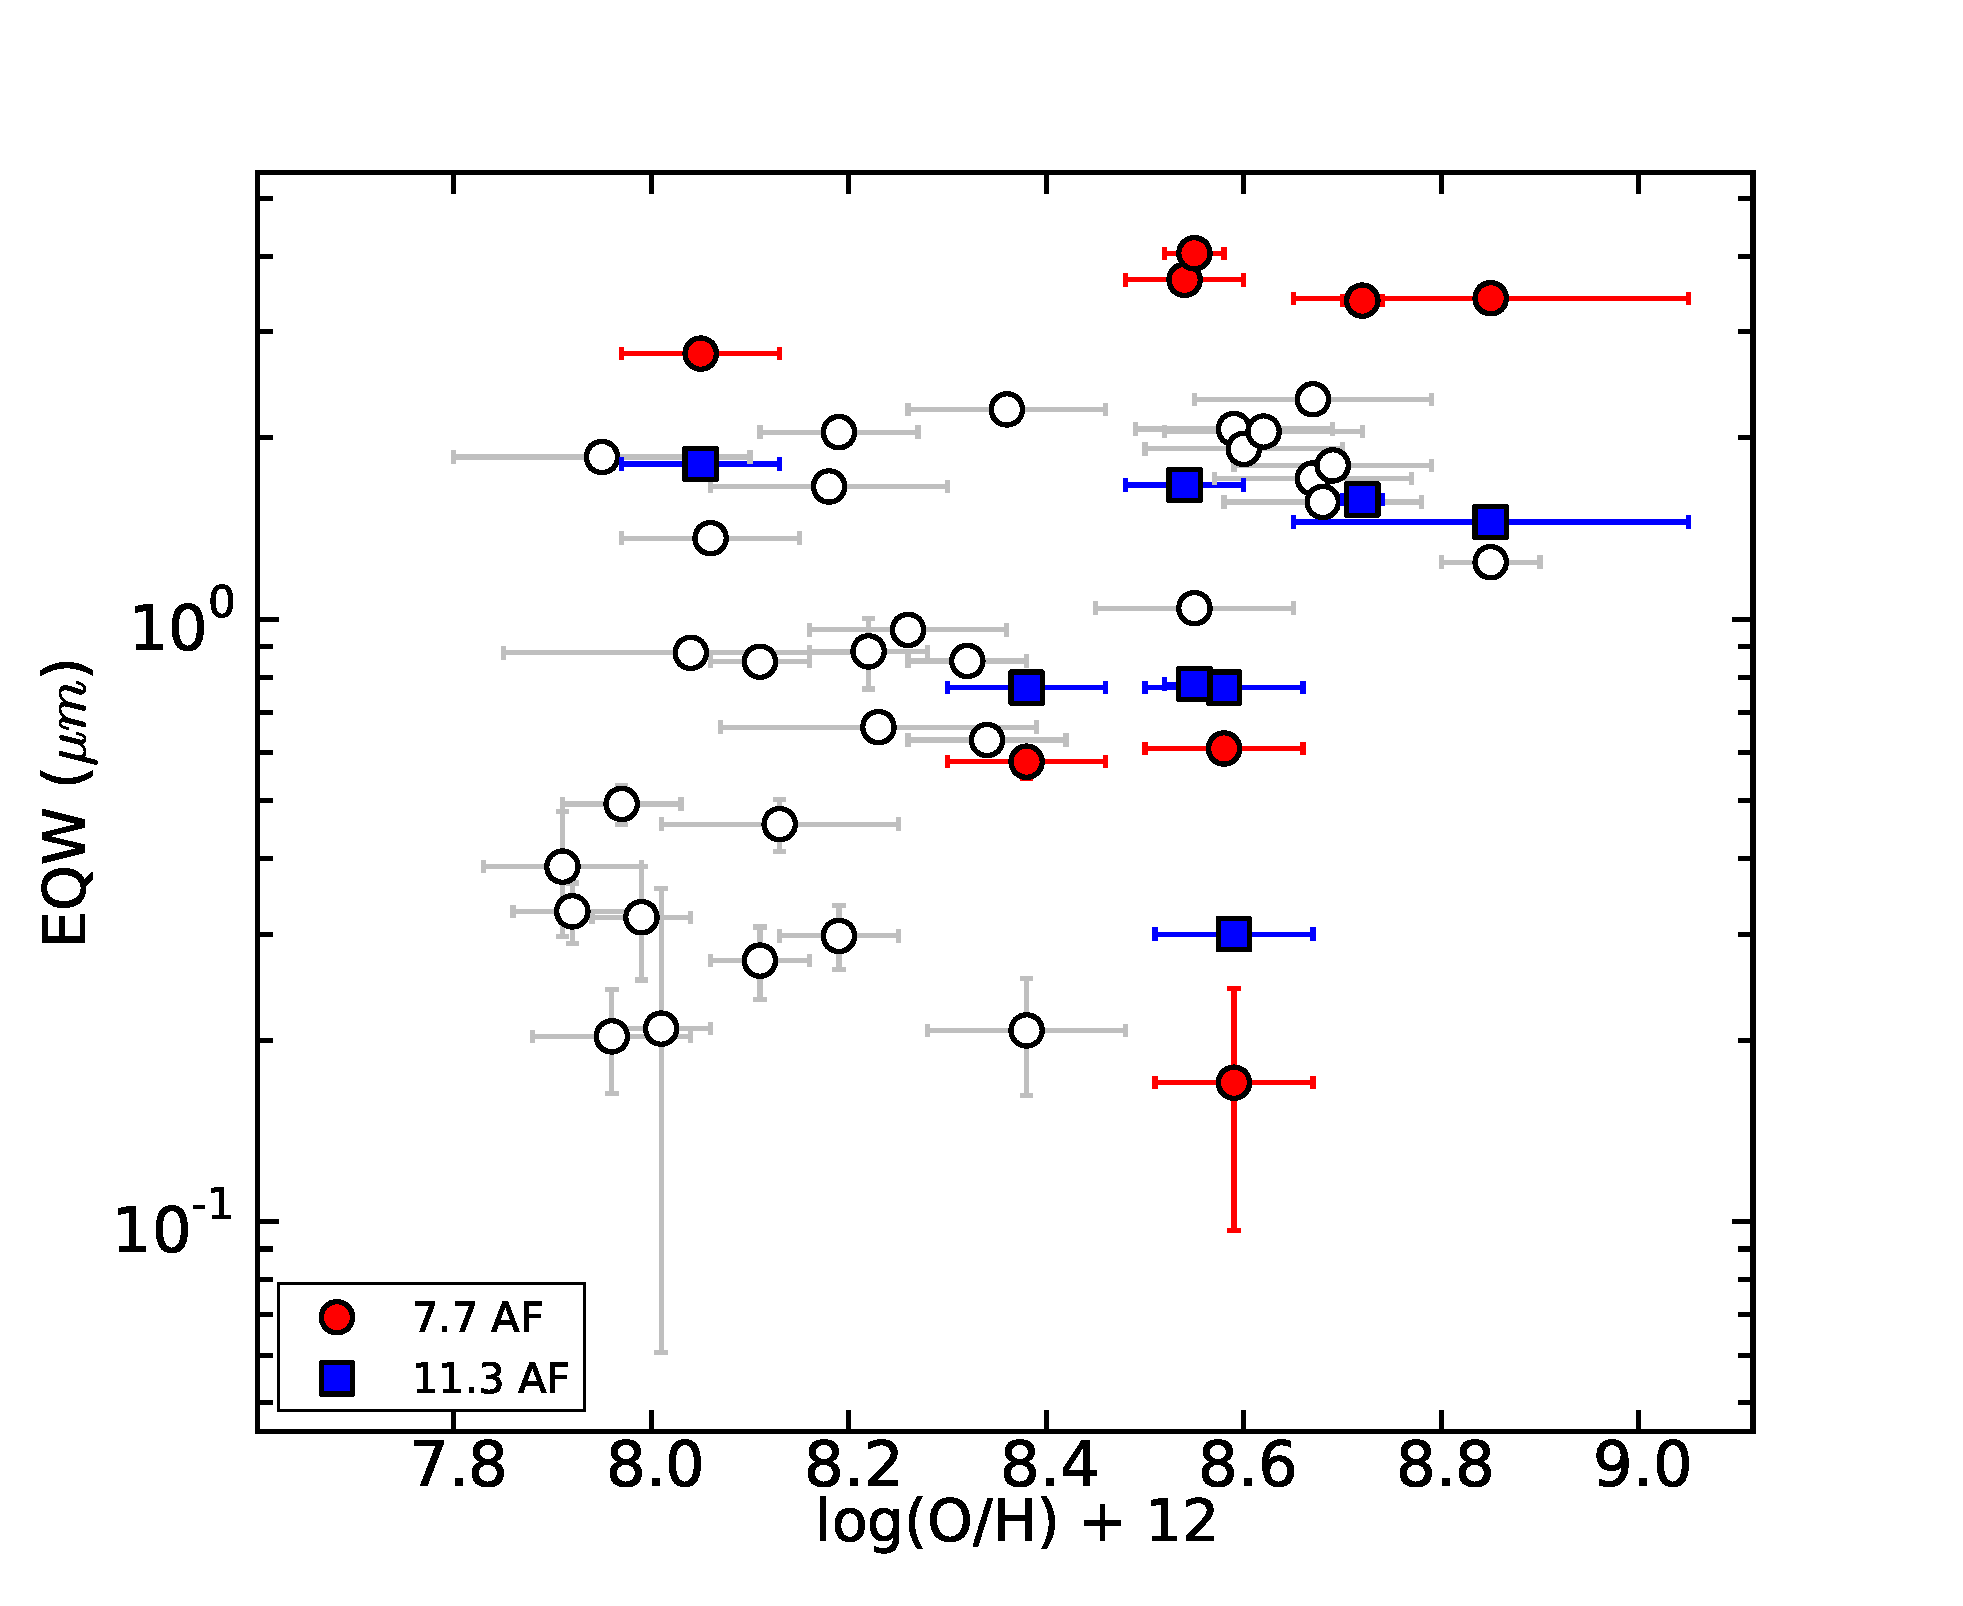
\includegraphics[scale=0.27]{./oxyvseqw.eps}
\caption{ PAH equivalent widths versus metallicity. EQWs of the 7.7~$\mu$m feature of the starburst sample from \citet{Engelbracht_2008} are plotted in open circles.}
\label{metalicityVseqw}
\end{figure}

The normalized EQWs of the PAH features are plotted versus the metallicity in our sample and the starburst galaxies of \citet{Engelbracht_2008}
 in Figure \ref{metalicityVseqw}. The metallicities in Engelbracht's work have been obtained by the direct electron temperature method 
 \citep{Skillman1998} whereas we used N06 N2 method. There is an offset between the metallicities generated by these two methods 
 since the N06 N2 method gives slightly higher values for the metallicity than the direct method. 
 This offset has been calculated by \citet{Mitchel2014} to be $0.35\pm0.10$. In Figure \ref{metalicityVseqw} we have corrected for this offset 
 by subtracting 0.35 from our metallicity values. 
	
Equivalent widths of the 7.7 and 11.3~$\mu$m features are not inconsistent with those of \citet{Engelbracht_2008}. However, we do not have enough data from low-metallicity regions in M31 to observe the expected decrease of EQWs of PAH with the decreasing metallicity.  There do seem to be some outliers which 
can plausibly be due to the uncertainties  and the offset between different methods of calculating the metallicity.  



\begin{figure}
\centering
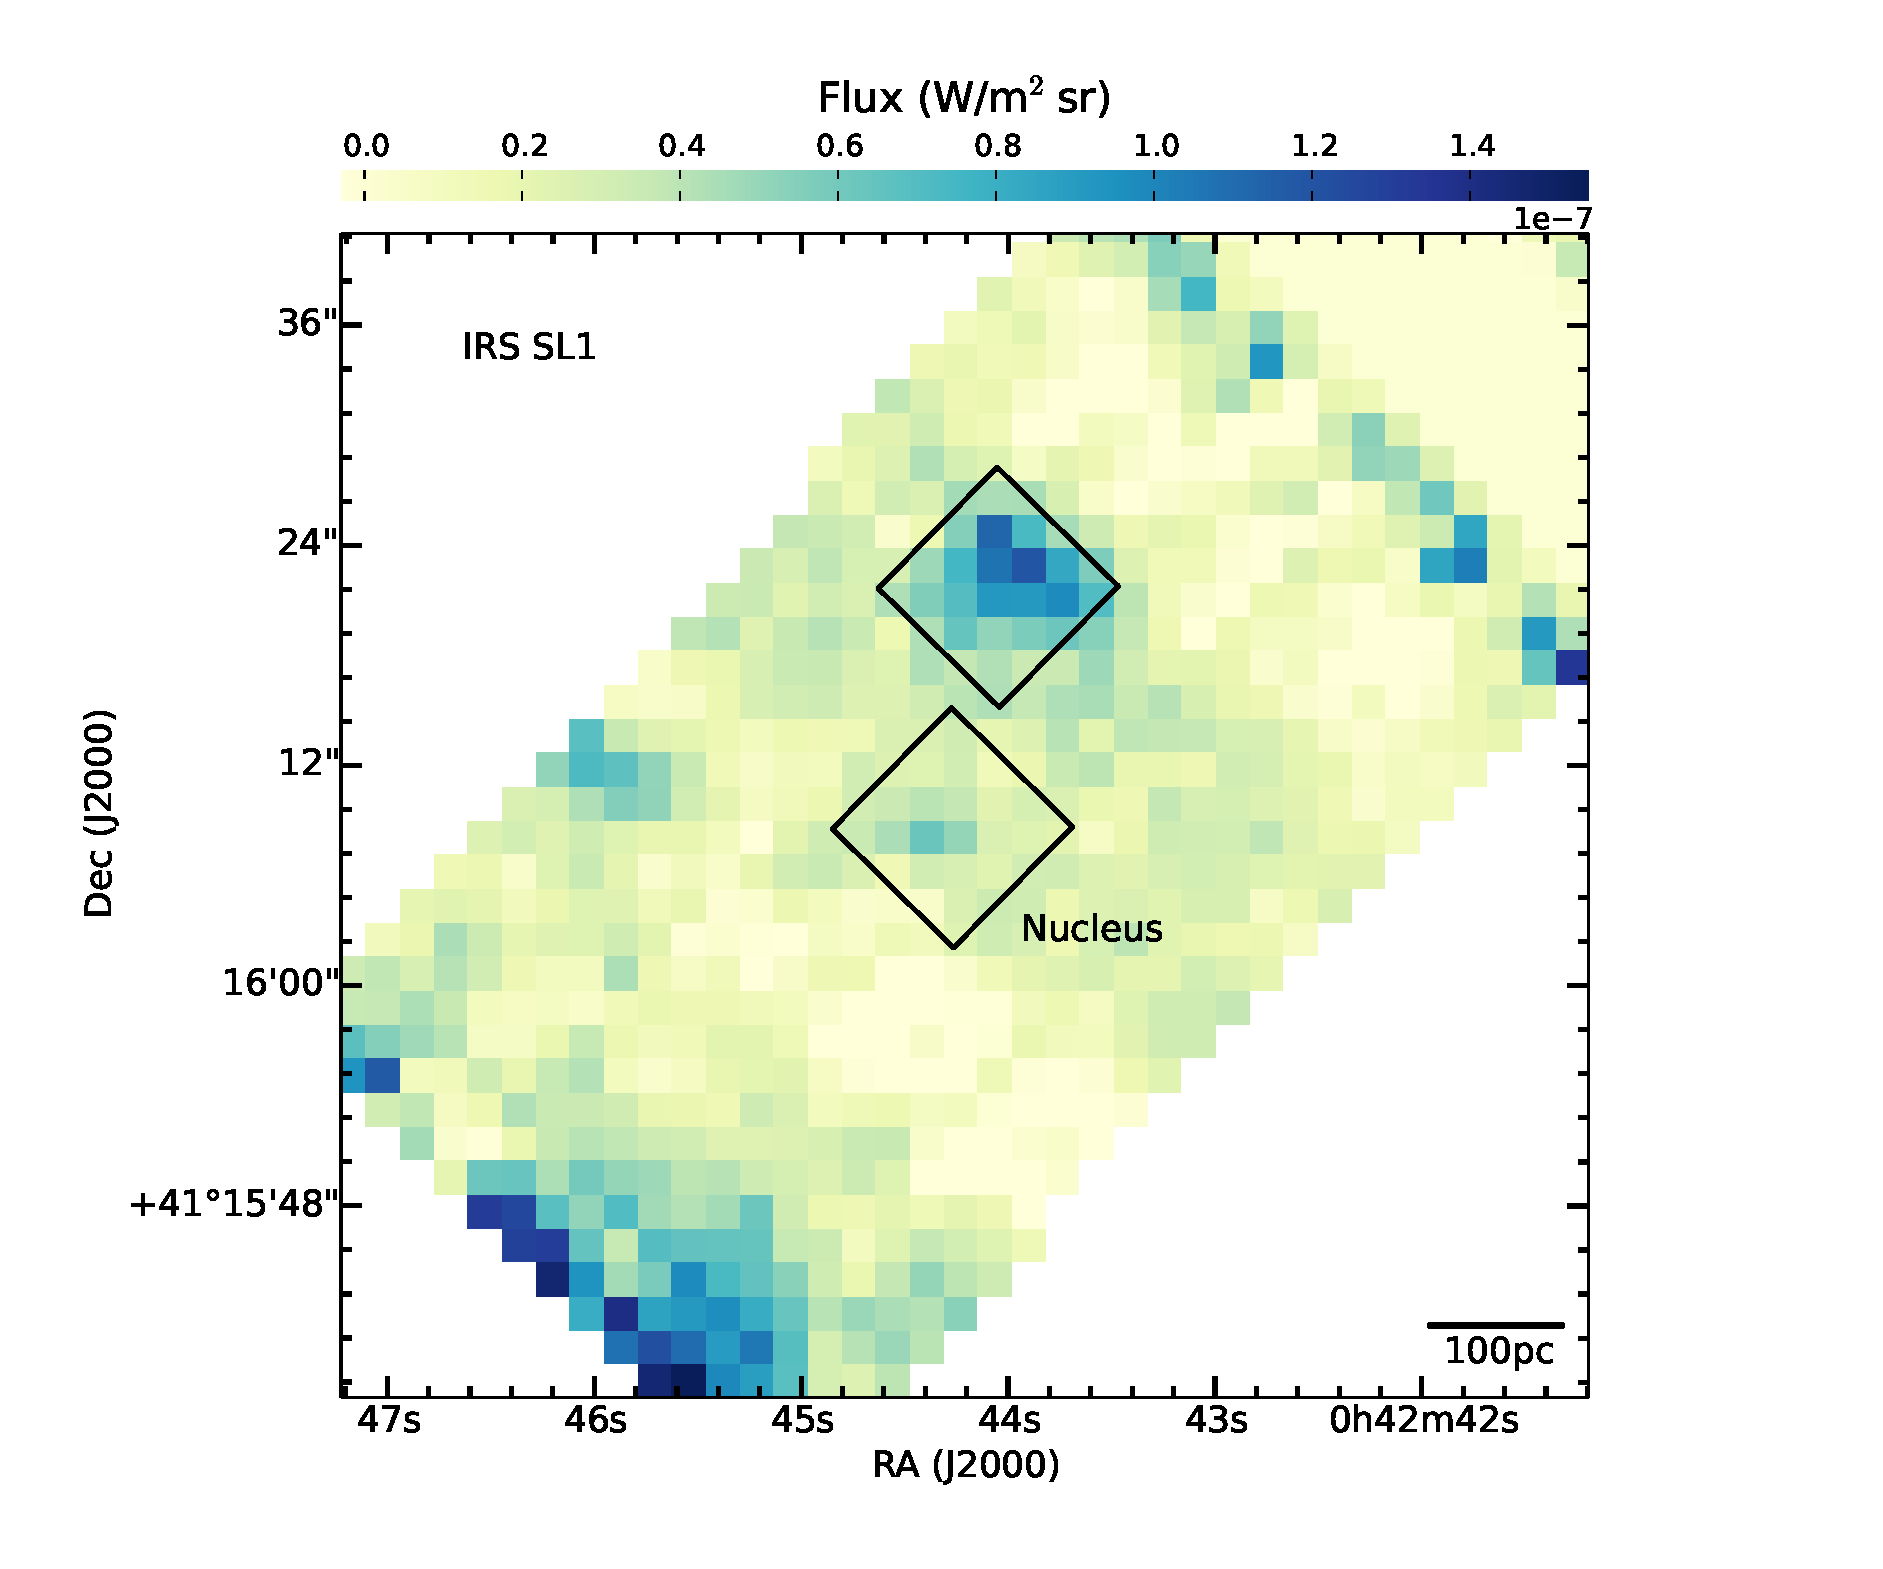
\includegraphics[width = 8 cm]{./nuc11_3.eps}
\caption{ Intensity variation of 11.3~$\mu$m emission around the nucleus of M31. 
Two black boxes are the apertures (centre and north region) used to extract spectra in Figure \ref{smithspec}. 
The centre of the nucleus is at R.A. 0h42m44.35s, Dec. +41d16m08.5s \citep{NucleusREF}.}
\label{nuc11}
\end{figure}

\subsection{Dust properties of the nucleus}
\label{sect:nucleus}

%HAS:
%First, let me call your attention to my paper on the IRS spectrum of M81, a LINER galaxy (Smith, H.A. et al. 2010)
%
%  http://adsabs.harvard.edu.ezp-prod1.hul.harvard.edu/cgi-bin/nph-data_query?bibcode=2010ApJ...716..490S&db_key=AST&link_type=ABSTRACT&high=485959d8d426165
%
%It has very strong silicate emission, and curiously resembles PG quasars in this respect. 
%We presume a hot dusty torus. We also image the dust around the nucleus; we see 11.3, 12.7 and 16.5 PAH, but only barely the 6.3 and 8.6 features. 
%
%I guess the nuclear spectrum is in your Figure 15 - why did you not try to fit it with PAHFIT too?  It looks to me like it has a weak 20um silicate bump too.
% Why not include the nuclear region in Tables 2,3&4?  I did not understand the reason for leaving it off.  Also please add the limit for the [Ne V] detection - it might still be a useful ratio with [Ne II] and the PAH lines.  It looked to me like there was some hint of the H2 12.28um line in some regions.... maybe add that limit too, though I was surprised

\begin{figure*}
\centering
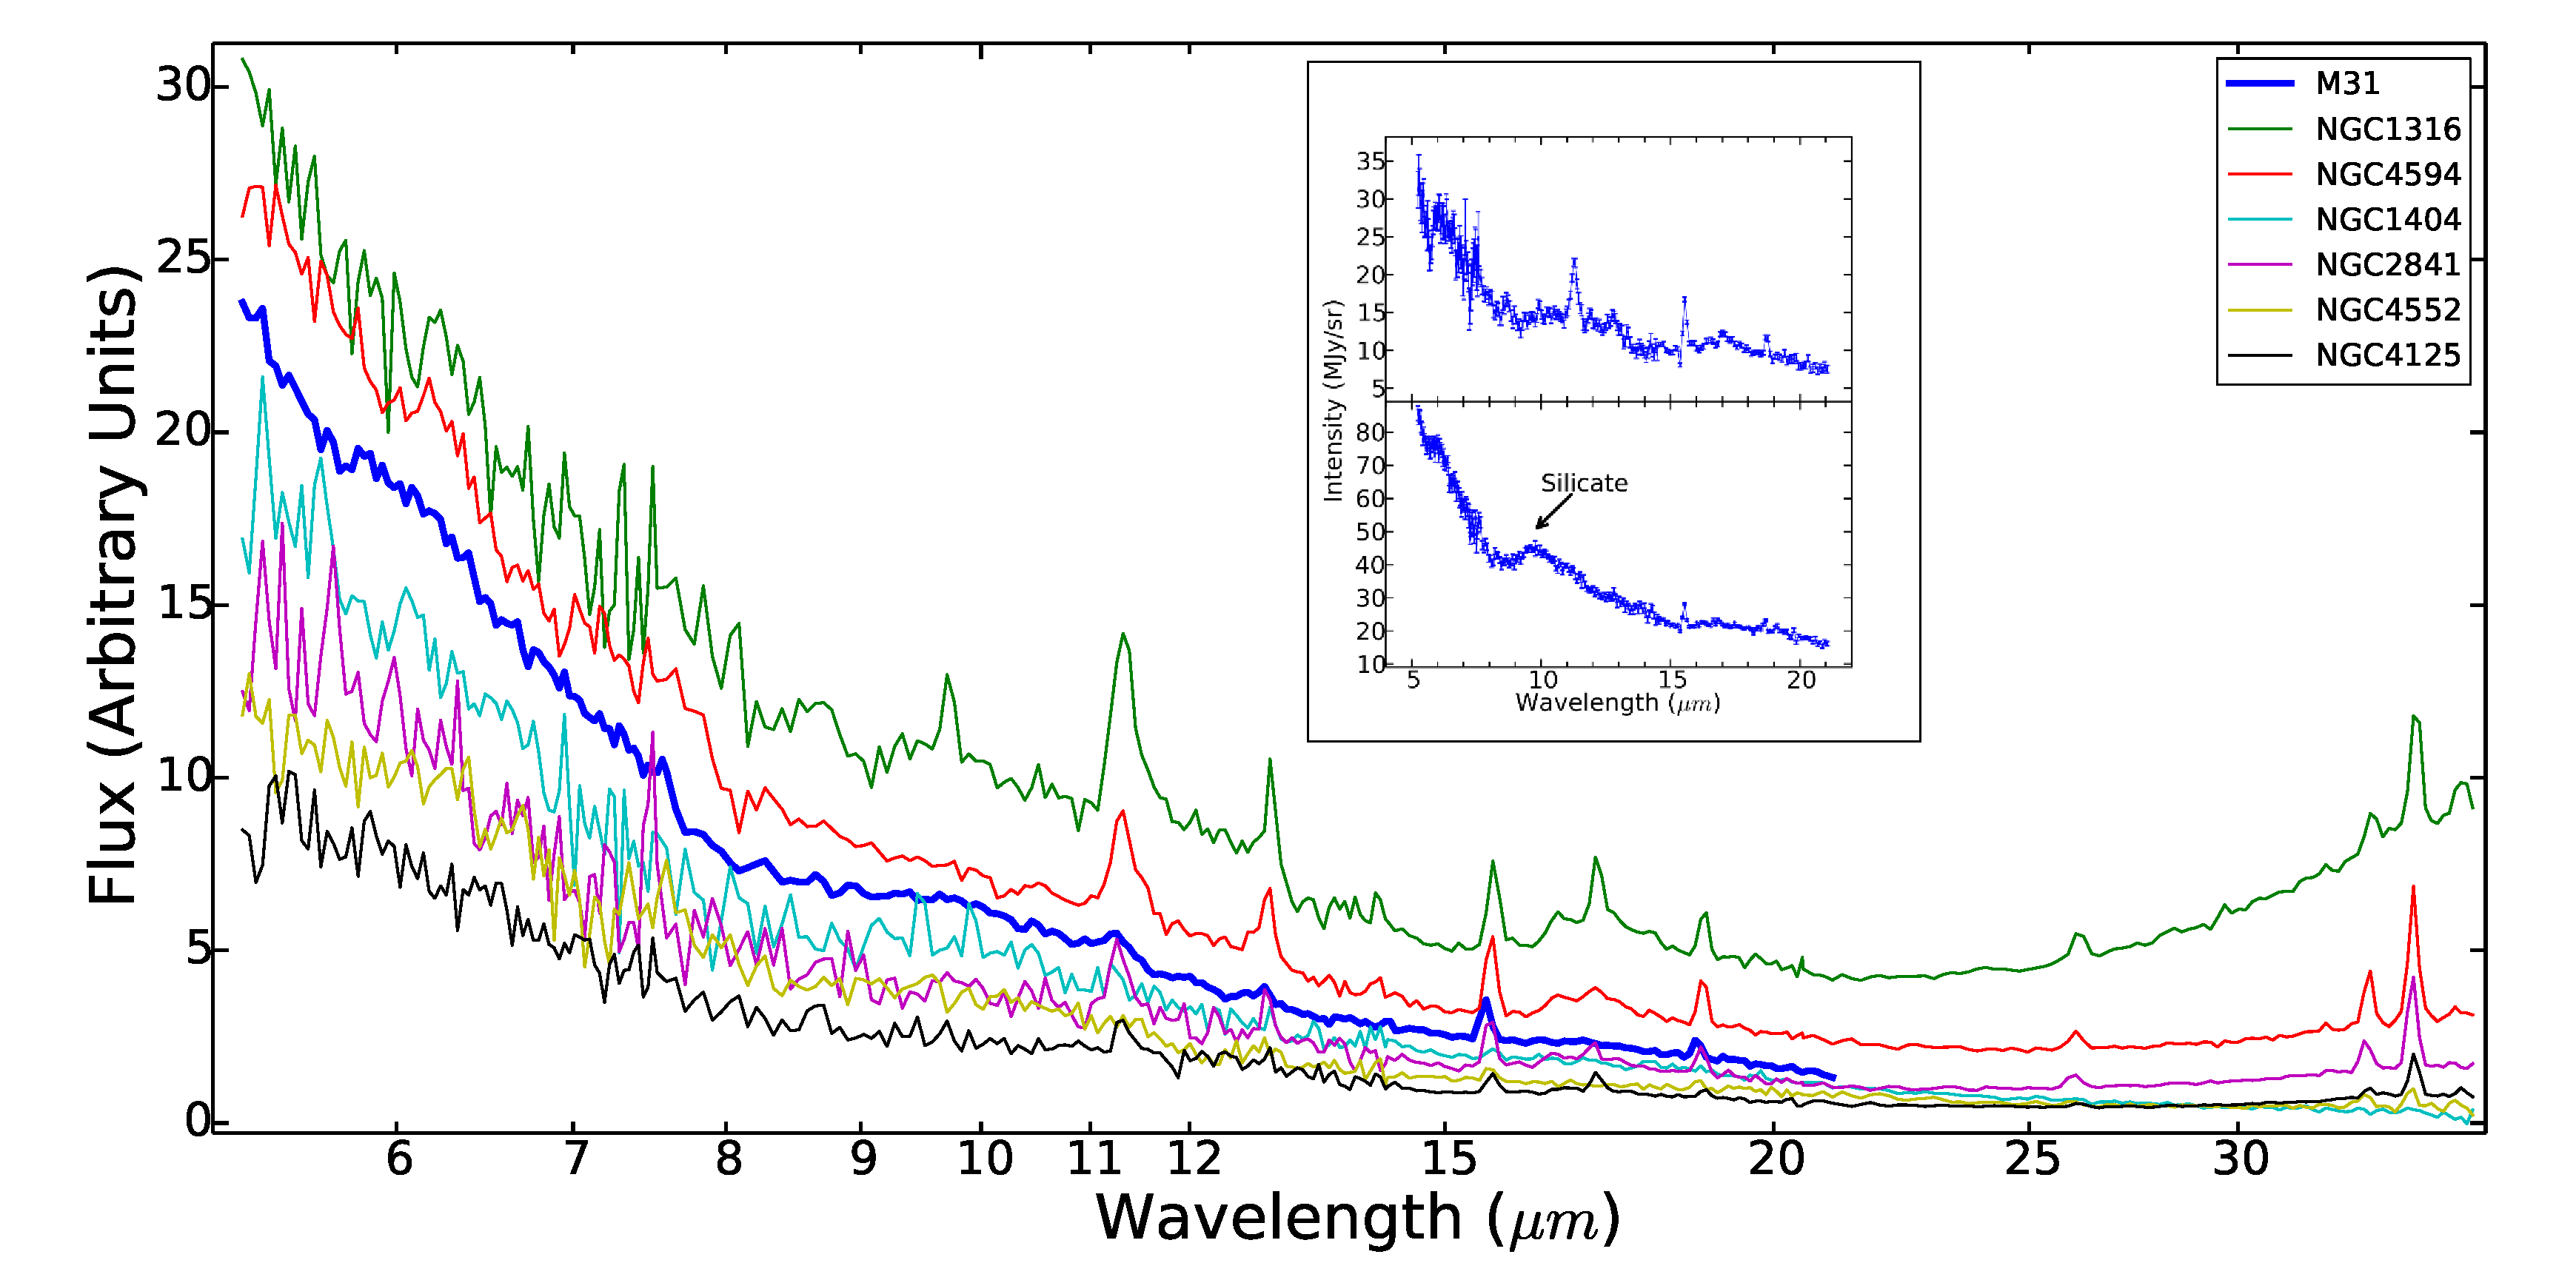
\includegraphics[height = 8 cm]{./SINGSspec.eps}
\caption{Mid-infrared spectrum of the nucleus of M31 (blue) over-plotted with spectra extracted close to the nuclei of 6 nearby galaxies which have 
AGN activity \citep{Smith:2007lr}. NGC 4552, NGC 1404 and NGC 4125 are elliptical galaxies and NGC 4594 and NGC 2841 are spiral galaxies. 
NGC 1316 is a lenticular galaxy. The inset shows the spectra extracted from the centre region of the M31 nucleus (bottom) and from the north region (top) 
shown in Figure \ref{nuc11}.}
\label{smithspec}
\end{figure*}

% HAS: On page 10, I think you might want to reference the black hole measuremts with HST of Bender et al  2005ApJ...631..280B.   
The centre of M31 has a complicated physical structure. It hosts a very inactive supermassive black hole with a mass of 
$0.7-1.4 \times 10^8$~M$_{\sun}$ \citep{Bacon2001} and it also has a lopsided nuclear disk \citep{Lauer1993} with two stellar components and an A-star cluster. 
The spectra of the nucleus from both {\em Spitzer} and ISOCAM show similar characteristics in the mid infrared wavelengths. 
Emission from the nucleus is missing the most common 6 to 8~$\mu$m PAH features while showing considerable emission around 11.3~$\mu$m. 

A suppression of 6 to 8~$\mu$m features has also been observed in other nearby star-forming galaxies with a low-luminosity AGN \citep{Smith:2007lr}. 
One explanation for this behaviour is that the AGN environment can selectively destroy the ionized or small PAH molecules which contribute to the 6 to 8~$\mu$m 
features (whereas larger, neutral PAHs contribute to the 11.3~$\mu$m feature). Another argument is that the AGN is unrelated or partially responsible for the PAH spectra alterations. \citet{Smith:2007lr} argue that this variation could be used to detect weak AGNs in dusty galaxies where optical diagnostics are not available. 
In Figure \ref{smithspec} we compare the spectrum of the nucleus of M31 with spectra extracted close to the nucleus of 6 other nearby galaxies and they 
all look very similar. All six galaxies are known to have low luminosity AGNs (LLAGNs) in the centre. Since M31 is showing a similar spectrum from the 
nucleus we can infer that  M31 also has a weak AGN at the centre.

Figure \ref{nuc11} shows the integrated intensity map of 11.3~$\mu$m emission around the nucleus. It can be observed that the majority of the 11.3~$\mu$m 
emission is coming from two regions (North and South East) around the centre of the nucleus and not from the centre. To study this further, we extracted two 
spectra, one from the centre and one from the North region using a $5 \times 5$ pixel square aperture as shown in Figure \ref{nuc11}. The spectrum extracted 
from the North region shows a strong 11.3~$\mu$m peak as expected and no considerable emission from 6 to 8~$\mu$m features (Figure \ref{smithspec}, inset). 
On the other hand the centre shows no PAH emission (Figure \ref{smithspec}) but silicate emission around 9.7~$\mu$m which is not present in the North spectrum. 
To investigate whether there are any other regions that show silicate emission close to the nucleus, a continuum subtracted image was produced which shows the 
9--11~$\mu$m integrated silicate emission intensity (see Figure \ref{silicate}). This silicate emission map shows that only the exact centre of the nucleus contributes 
to the silicate emission. 

\citet{Spoon2007} report that galaxies which have AGN activity show silicate emission around 9.7~$\mu$m.
In the unified model of AGNs, an edge on view through cool dust (type 2 AGNs) in the torus causes silicate absorption whereas a face-on view (type 1 AGNs) 
shows silicate emission \citep{AGNtypes1995}. The latter could be the reason for silicate emission of M31 if it holds a Seyfert-like AGN. 
But the mid-IR spectra do not contain forbidden atomic lines such as [Ne~{\sc v}] and [S~{\sc iv}] which are indicative of such an active nucleus \citep{AGNref}.

 Alternatively, the silicate emission is not directly associated with the torus but rather originate in the optically thin hot dust around the torus \citep{Mason2012}. 
 The first detection of such silicate emission is reported in \citet{Sturm2005} from the low-ionization nuclear emission-line region (LINER) galaxy NGC 3998. 
 LINERs are powered by accretion onto massive black holes and due to the low accretion rates these are classified as the low-luminosity AGNs \citep{Kewley2006}. 
 \citealt{Mason2012} has observed that this 9.7~$\mu$m silicate emission is present in many LLAGNs. They also have explained that these objects cannot 
 host a Seyfert-like obscuring torus because of their optically thin dust and low dust-to-gas ratio. By taking all these into account, we can suggest that M31 
 hosts a low-luminosity AGN. 

%HAS: I was trying to think more about the significance of the result. Although indeed some quasars and LINERS have silicate emission, I don't think your conclusion in the abstract that the emission "provides evidence for a LLAGN" is correct as worded -  3C273 has silicate emission too.  It might be useful to tabulate the masses of the black holes in each of the 6 comparison galaxies, to see whether spectral similarities (or differences) can be attributed to the quiescent AGN, as you suggest, of whether circumnuclear star formation or other things might play some role.
 
Also, the bolometric luminosity of the nucleus was calculated to be (value goes here erg/ s) using the 12~$\mu$m flux using the method described in \citet{luminosity}. This value is closer to that of other LLAGNs.


\begin{figure}
\centering
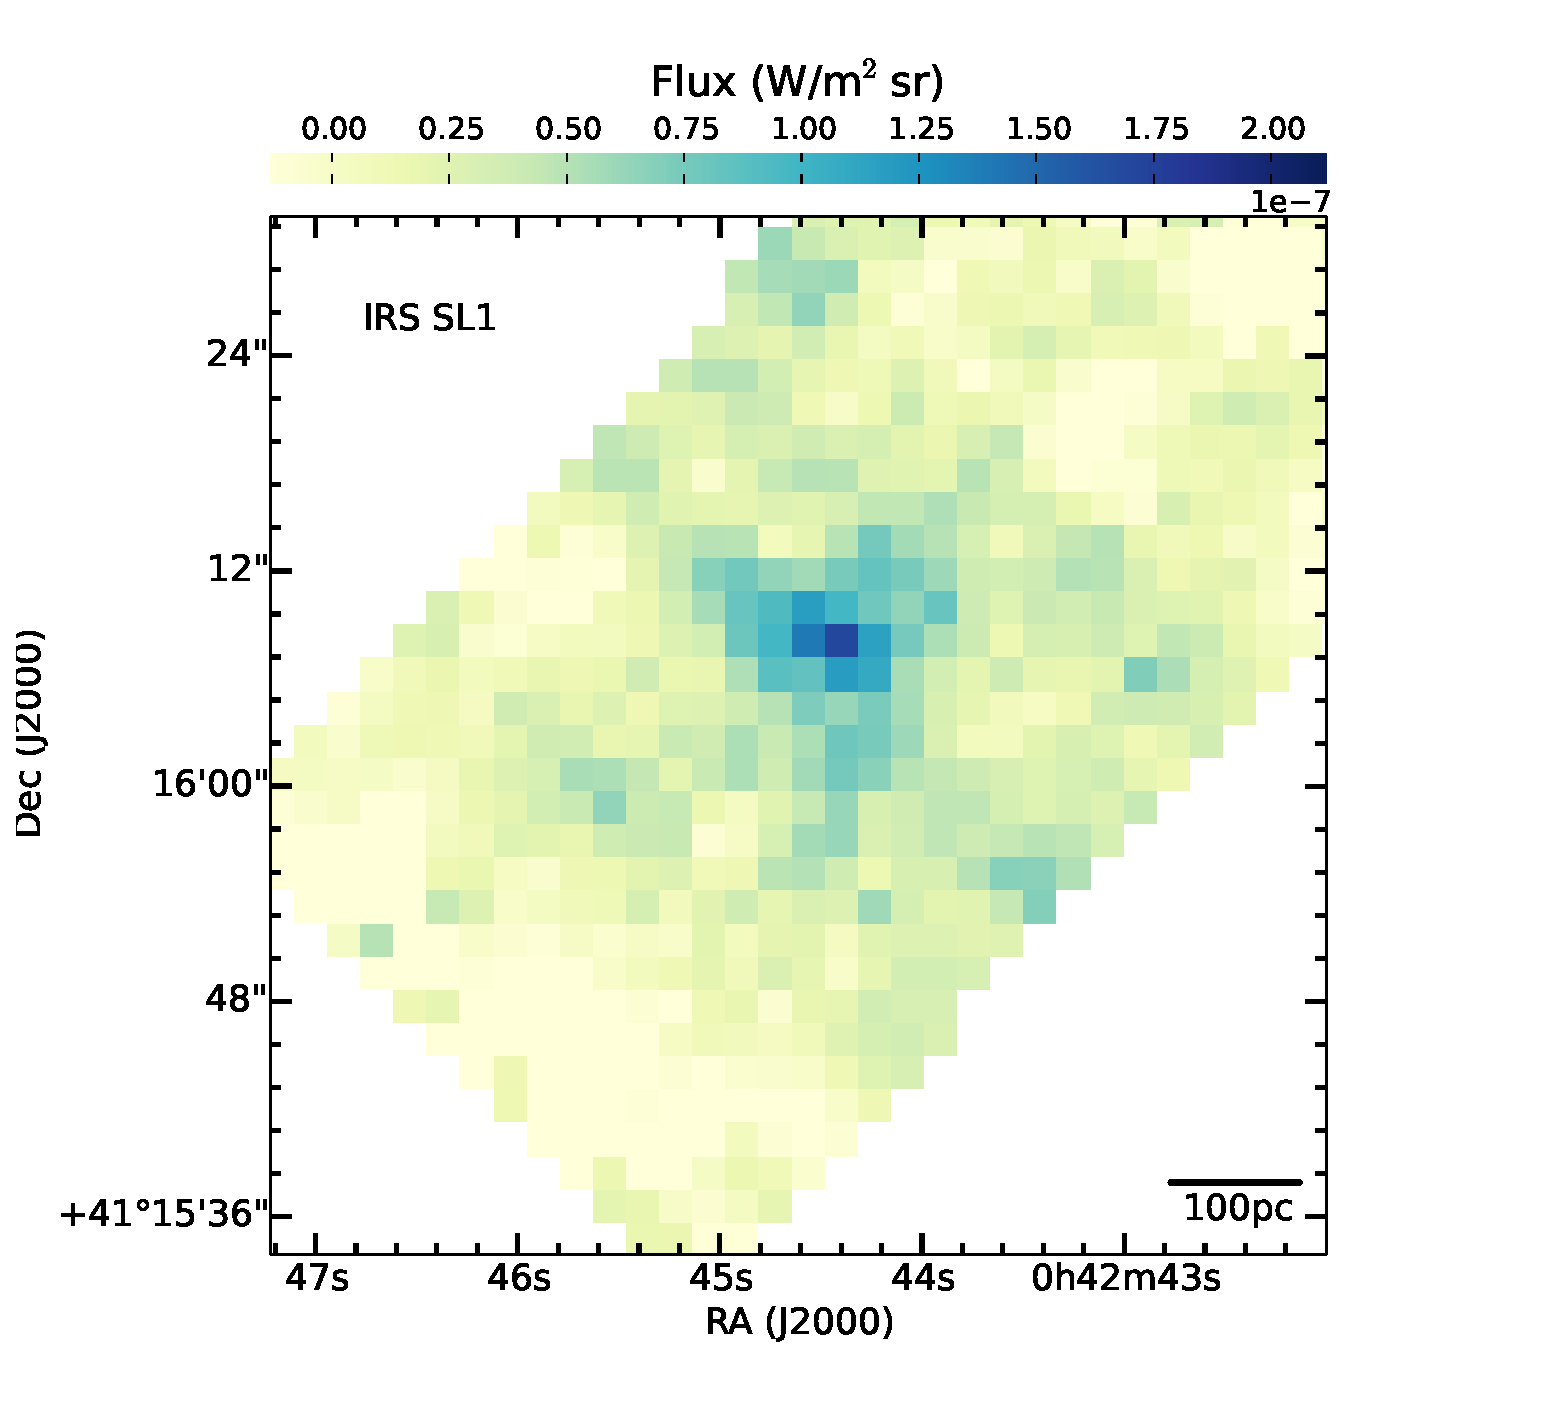
\includegraphics[scale = 0.3]{./NUCsilicate.eps}
\caption{The integrated strength of the silicate emission (from 9 to 11~$\mu$m) near the M31 nucleus.}
\label{silicate}
\end{figure}
